\emph{
	Escriba dos programas en Octave que simulen al proceso de Poisson 
	de par\'ametro $\lambda$ en el intervalo $[0,1]$. En uno utilizar\'a 
	s\'olo variables exponenciales y en el otro puede utilizar una 
	variable Poisson.
}

Utilizando variables de distribución exponencial para los 
saltos:\pn

\small
\texttt{
	\lstinputlisting[inputencoding=utf8]{tarea5/problema5_1/ProcesoPoissonConExponenciales.m}
}
\normalsize

A continuación una gráfica obtenida de ejecutar este código:\pn
\begin{center}
    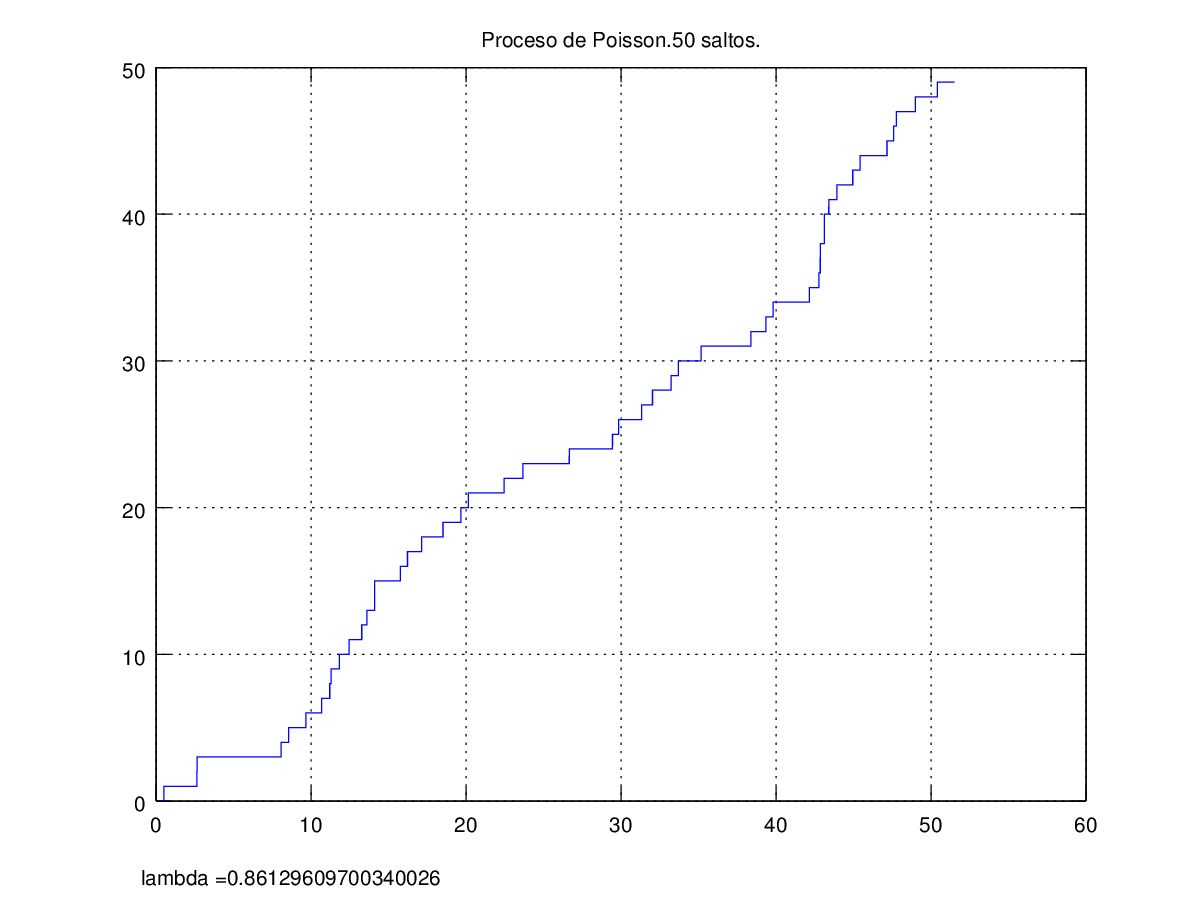
\includegraphics[width=8cm]{tarea5/problema5_1/ProcesoPoissonConExponenciales.png}
\end{center}

La implementación anterior fue hecha intentando representar el proceso de Poisson de parámetro
$\lambda$ durante los $50$ primeros saltos.

\newpage

Utilizando variables de distribución Poisson para determinar 
la cantidad de saltos hasta el tiempo $t$:\pn

\small
\texttt{
	\lstinputlisting[inputencoding=utf8]{tarea5/problema5_1/ProcesoPoissonConPoisson.m}
}
\normalsize

A continuación una gráfica obtenida de ejecutar este código:\pn

\begin{center}
    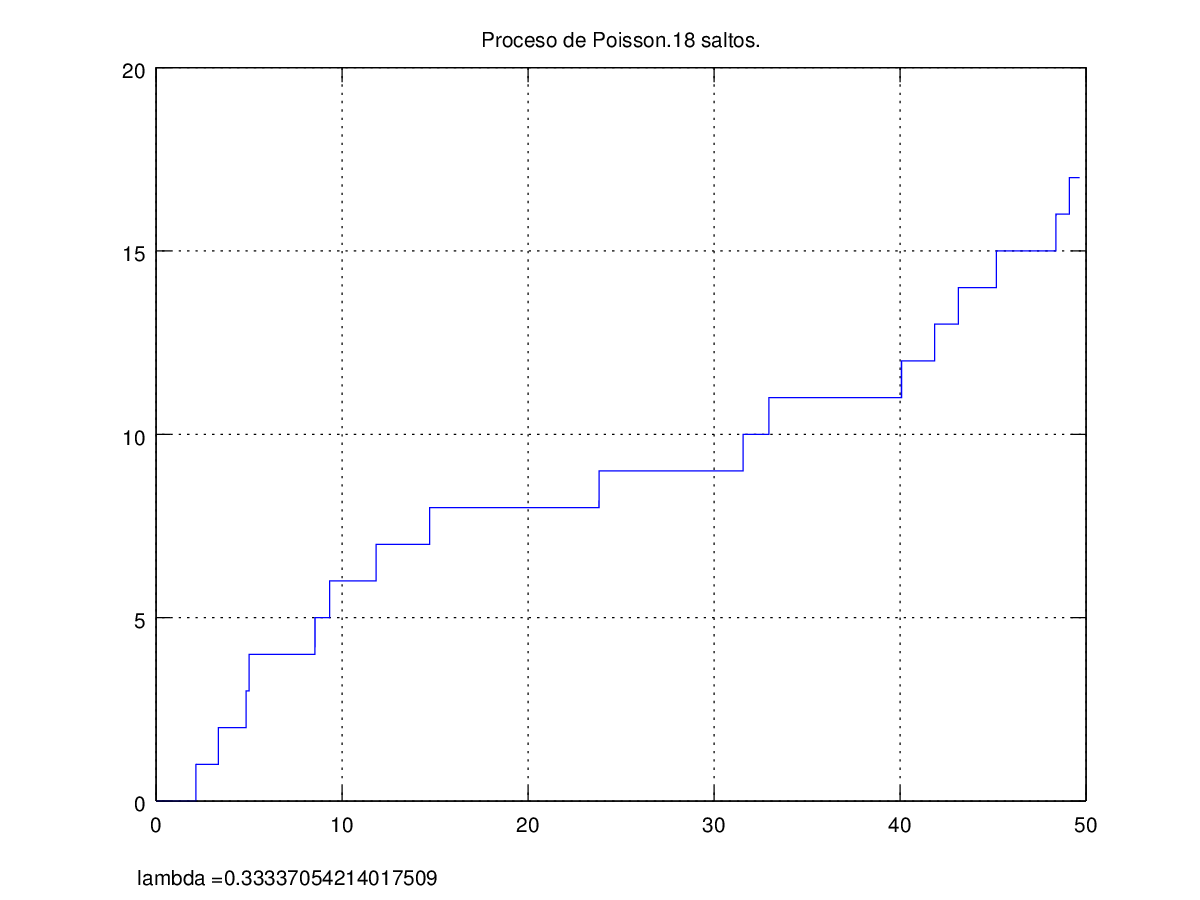
\includegraphics[width=8cm]{tarea5/problema5_1/ProcesoPoissonConPoisson.png}
\end{center}

A diferencia de la implementación anterior, esta vez intentamos representar el proceso de Poisson 
hasta un tiempo dado y no hasta un número de saltos dado. \pn

Como se puede apreciar, en esta última ejecución hasta el tiempo $50$ únicamente hubo $18$ saltos. 
A diferencia de que en la ejecución de la primera implementacción hubo $43$ saltos para el 
tiempo $50$. Cabe notar, que el parámetro lambda de la primera implementación era aproximadamente 
$0.915432$, mientras que el de la segunda a penas aproximadamente $0.333371$. Hay que recordar
que los ``holding times'' tienen distribución exponencial, tienden a ser más largos 
conforme $\lambda$ es más pequeño, y por lo tanto, entre más pequeño sea, habrá saltos con menos frecuencia.\pn

\textbf{Nota: } Para poder implementar esta versión del algoritmo se necesitó implementar
una función que se deduce del resultado de [\ref{problema5_1:inciso3}]. Esta parte está en el archivo con nombre
\texttt{t1\_dado\_tn\_rnd.m}. Esta función se usa para calcular los tiemos de salto y lo único
que hace es simular una variable aleatoria con la densidad del resultado de [\ref{problema5_1:inciso3}].